\documentclass{article}

% Language setting
% Replace `english' with e.g. `spanish' to change the document language
\usepackage[T2A]{fontenc}
\usepackage[utf8]{inputenc}

% Set page size and margins
% Replace `letterpaper' with `a4paper' for UK/EU standard size
\usepackage[letterpaper,top=2cm,bottom=2cm,left=3cm,right=3cm,marginparwidth=1.75cm]{geometry}

% Useful packages
\usepackage{amsmath}
\usepackage{graphicx}
\usepackage{float}
\usepackage[colorlinks=true, allcolors=blue]{hyperref}
\usepackage{biblatex}
\usepackage{arabicore}

\title{Лабораторная работа №3}
\author{Выполнили: Цалов В.С. Тахватулин М.В.}

\begin{document}
\maketitle
\begin{center}
      {\fontsize{14}{15}\selectfont
            Преподователь: Оранский С.И.
      }
\end{center}
\section{Задание 1}
\subsection{Условие}
С помощью критерия согласия Пирсона хи-квадрат проверить согласованность
рейтинг футболиста с нормальным законом. Ту же самую задачу решить с помощью другого
критерия
\subsection{Выполнение}
Гипотезы: 
\begin{itemize}
      \item $H_0$: рейтинг футболистов распределен по нормальному закону
      \item $H_1$: рейтинг футболистов распределен по не норамльному закону
\end{itemize}
Алгоритм выполнения
\begin{enumerate}
      \item Суммируем рейтинг, чтобы получить величину
      \item Далее находим среднее и отклонение данной выборки
      \item Делаем выборку интервальной
      \item По найденым ранее параметра находим ожидаемые значения
      \item Находим $ \chi^2_{\text{набл}} $ и $ \chi^2_{\text{набл}} $
      \item Сравниваем их и определяем верную гипотезу
      \item Также проверяем гипотезы с помощью критерия Колмогорова-Смирнова
\end{enumerate}
\subsection{Вывод программы}
Наблюдаемое значение хи-квадрат критерия: 11172.965189630037 \\ 
Критическое значение хи-квадрат критерия: 22.362032494826934 \\ 
Есть основания отвергать гипотезу $H_0$ $\rightarrow$ 1 гипотеза (ненормальное распределение) \\
Критерий Колмогорова-Смирнова:
Есть основания отвергать гипотезу $H_0$ $\rightarrow$ выборка распределена по не нормальному закону

\begin{figure}[H]
      \centering
      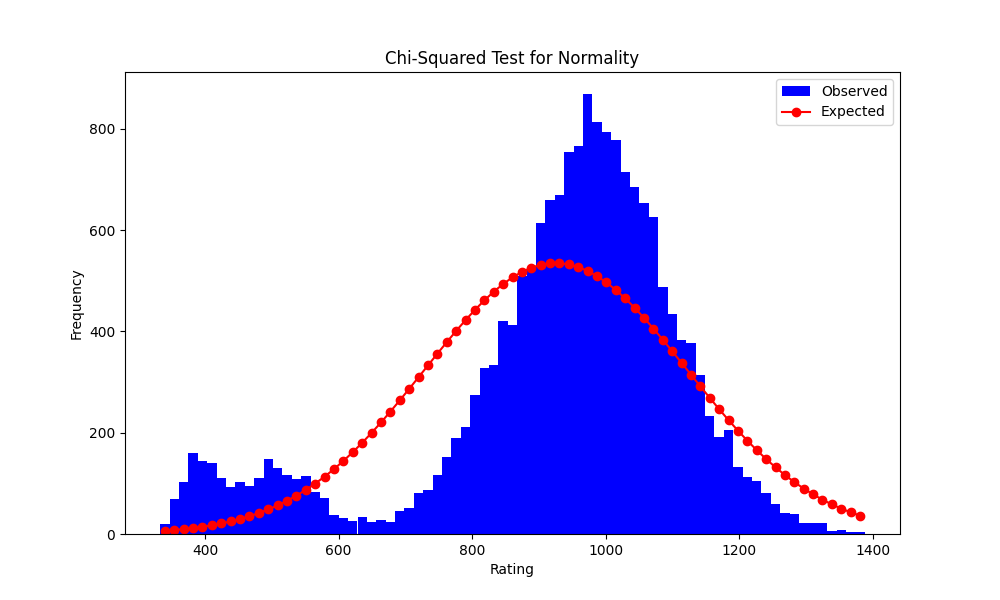
\includegraphics[width=1\linewidth]{../python/task1.png}
      \caption{Гистограмма распределения футболистов и ожидаемое нормальное распределение с полученными параметрами}\label{fig:figure1}
\end{figure}
\subsection{Выводы}
Как критерий хи-квадрат, так и критерий Колмогорова-Смирнова опровергли гипотезу о том, что выборка рейтинга основана на нормальном законе. Также из графика видно, что это действительно так.

\section{Задание 2}
\subsection{Условие}
С помощью критерия однородности хи-квадрат проверить однородность рейтинга молодых и возрастных футболистов. Ту же самую задачу решить с помощью другого критерия
\subsection{Выполнение}
Гипотезы:
\begin{itemize}
      \item $H_0$: рейтинг молодых и возрастных футболистов однороден
      \item $H_1$: рейтинг молодых и возрастных футболистов не однороден 
\end{itemize}
Алгоритм выполнения:
\begin{enumerate}
      \item Делим футболистов по возрасту
      \item Разбиваем две выборки на интервалы
      \item После этого находим наблюдаемое и критическое значения
      \item Сравниваем их и опрделяем верную гепотезу
      \item Делаем тоже самое с помощью критерия Колмогорова-Смирнова
\end{enumerate}
\subsection{Вывод программы}
Проверка гипотезы о том, что выборки молодых и возрастных футболистов однородны: \\
наблюдаемое значение критерия: 601.6660440175403 \\ 
критическое значение критерия: 4922.634987383697 \\ 
нет оснований отвергать нулевую гипотезу $ \rightarrow $ выборки однородны \\ 
Проверка гипотезы о том, что выборки молодых и возрастных футболистов однородны с помощью критерия Колмогорова-Смирнова: \\ 
Статистика Колмогорова-Смирнова: 0.12954988393062894 \\
p-значение: 1.364126296813217e-44 \\ 
Отвергаем нулевую гипотезу: выборки неоднородны.  \\
\begin{figure}[H]
      \centering
      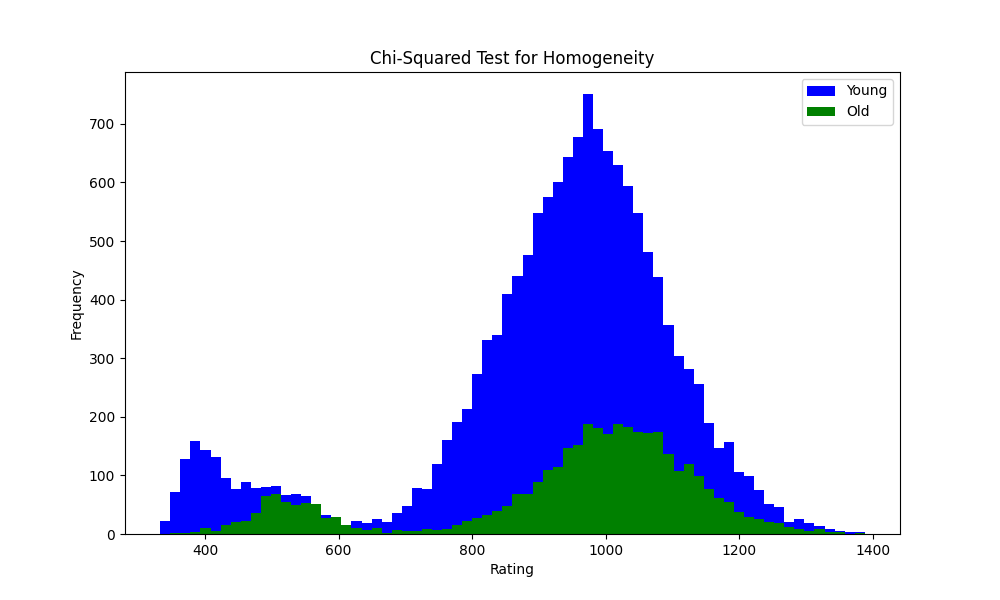
\includegraphics[width=1\linewidth]{../python/task2.png}
      \caption{Гистограмма распределения футболистов и ожидаемое нормальное распределение с полученными параметрами}\label{fig:figure}
\end{figure}
\subsection{Выводы}
Мы получили неоднозначный результат. Критерий хи-квадрать принимает гипотезу, а критерий Колмогорова-Смирнова отвергает.


\section{Задание 3}
\subsection{Условие}
С помощью критерия независимости хи-квадрат проверить независимость рейтинга и национальности футболиста. Ту же самую задачу решить с помощью другого критерия
\subsection{Выполнение}
Гипотезы:
\begin{itemize}
      \item $H_0$: Значения рейтинга зависят от национальности
      \item $H_1$: Значения рейтинга не зависят от национальности
\end{itemize}
Алгоритм выполнения:
\begin{enumerate}
      \item Составляем таблицу сопряженности
      \item Разбиваем колноку рейтинга на интервалы
      \item Находим наблюдаемое и критическое значение критерия
      \item Сравниваем и определяем гипотезу
\end{enumerate}
\subsection{Вывод программы}
Наблюдаемое значение хи-квадрат критерия: 5002.698494943362
Критическое значение хи-квадрат критерия: 2499.7277366742187
Гипотеза $H_0$ отвергается $\rightarrow$ значения рейтинга не зависят от национальности

\subsection{Код}
      \begin{verbatim}
import math
import numpy as np
import pandas as pd
import scipy.stats as stats
import matplotlib.pyplot as plt

data = pd.read_csv('fifa_players_stats.csv', delimiter=",", skiprows=1, names=[
    'Known As', ...,   'GK Rating'])

data['total_rating'] = data['ST Rating'] + data['LW Rating'] + data['LF Rating'] + \
                              data['CF Rating'] + \
                       data['RF Rating'] + data['RW Rating'] + data['CAM Rating'] + \
                       data['LM Rating'] + data['CM Rating'] + data['RM Rating'] + \
                       data['LWB Rating'] + data['CDM Rating'] + data['RWB Rating'] + \
                       data['LB Rating'] + data['CB Rating'] + \
                       data['RB Rating'] + data['GK Rating']


# С помощью критерия согласия Пирсона хи-квадрат проверить согласованность
# рейтинг футболиста с нормальным законом (формализовать основные и альтернативные ги-
# потезы, реализовать самостоятельно).

# гипотезы:
# 0 гипотеза - нормальное распределение
# 1 гипотеза - не нормальное распределение
def task1(data):
    # Ожидаемые значения
    srednee = data['total_rating'].mean()
    otklonenie = data['total_rating'].std()

    observed, bins = np.histogram(data['total_rating'], bins='auto')
    expected = np.array([stats.norm.cdf(bins[i + 1], srednee, otklonenie) -
                         stats.norm.cdf(bins[i], srednee, otklonenie) for i in
                         range(len(bins) - 1)]) * len(data['total_rating'])
    expected = expected * (observed.sum() / expected.sum())

    xi_square_nabl = ((observed - expected) ** 2 / expected).sum()
    print(f'наблюдаемое значение хи-квадрат критерия: {xi_square_nabl}')
    xi_square_crit = stats.chi2.ppf(0.95, math.ceil(math.log2(data.shape[0])+1)-3)
    print(f'критическое значение хи-квадрат критерия: {xi_square_crit}')




    plt.figure(figsize=(10, 6))
    plt.hist(data['total_rating'], bins=bins, label='Observed', color='blue')
    plt.plot((bins[1:] + bins[:-1]) / 2, expected, 'o-', label='Expected', color='red')
    plt.xlabel('Rating')
    plt.ylabel('Frequency')
    plt.title('Chi-Squared Test for Normality')
    plt.legend()
    plt.show()

    if xi_square_crit > xi_square_nabl:
        print(f"0 гипотеза (нормальное распределение)")
    else:
        print(f"1 гипотеза (ненормальное распределение)")

    KolmonSmin_rating(data)

    return xi_square_nabl

# Ту же самую задачу решить с помощью другого
# критерия (тоже формализовать гипотезы, но здесь можно воспользоваться готовой реализацией)
def KolmonSmin_rating(data):
    print("\n")
    print("Критерий Колмогорова-Смирнова")
    # Проверяем выборку на нормальность c помощью критерия Колмогорова-Смирнова
    statistic, pvalue = stats.kstest(data["total_rating"], 'norm')

    # Уровень значимости
    alpha = 0.05
    if pvalue > alpha:
        print("Гипотеза о нормальности распределения не отвергается.")
    else:
        print("Гипотеза о нормальности распределения отвергается.")


# Задание 2: Проверка однородности и построение графика
def task2(data, age):
    print("\n")
    print("Проверка гипотезы о том, что выборки молодых и возрастных футболистов однородны:")
    # Гипотеза 0 - выборки молодых и возрастных футболистов однородны
    # Гипотеза 1 - выборки молодых и возрастных футболистов не однородны

    young = data[data['Age'] < age]['total_rating']
    old = data[data['Age'] >= age]['total_rating']

    observed_young, bins = np.histogram(young, bins='auto')
    observed_old, old_bins = np.histogram(old, bins=bins)
    observed_young = observed_young * (observed_old.sum() / observed_young.sum())
    count_str_1 = observed_young.shape[0]
    count_str_2 = observed_old.shape[0]

    xi_square_nabl = stats.chi2_contingency([observed_young, observed_old])[0]
    # xi_square_nabl = stats.chi2_contingency([young, old])[0]
    print(f'наблюдаемое значение критерия: {xi_square_nabl}')

    # подсчёт количества степеней свободы
    df = (count_str_1 - 1) * (count_str_2 - 1)
    xi_square_crit = stats.chi2.ppf(0.95, df)
    print(f'критическое значение критерия: {xi_square_crit}')

    plt.figure(figsize=(10, 6))
    plt.hist(young, bins=bins, label='Young', color='blue')
    plt.hist(old, bins=bins, label='Old', color='green')
    plt.xlabel('Rating')
    plt.ylabel('Frequency')
    plt.title('Chi-Squared Test for Homogeneity')
    plt.legend()
    plt.show()

    if xi_square_crit > xi_square_nabl:
        print("нет оснований отвергать нулевую гипотезу -> выборки однородны")
    else:
        print("есть основания отвергать нулевую гипотезу -> выборки не однородны")

    KolmonSmin_age(young, old)

    return xi_square_nabl

def KolmonSmin(sample1, sample2):
    # Критерий Колмогорова-Смирнова
    statistic, pvalue = stats.ks_2samp(sample1, sample2)


    print("\n")
    print("Проверка гипотезы о том, что выборки молодых и возрастных футболистов однородны с помощью критерия" +
            + "Колмогорова-Смирнова:")
    print(f"Статистика Колмогорова-Смирнова: {statistic}")
    print(f"p-значение: {pvalue}")

    alpha = 0.05
    if pvalue < alpha:
        print("Отвергаем нулевую гипотезу: выборки неоднородны.")
    else:
        print("Нет оснований отвергать нулевую гипотезу: выборки однородны.")

# Задание 3: Проверка независимости и построение графика
def task3(data):

    k = math.ceil(math.log2(data.shape[0]) + 1)

    contingency_table = pd.crosstab(data['Nationality'], pd.cut(data['total_rating'], k))

    row_sums = contingency_table.sum(axis=1)
    col_sums = contingency_table.sum(axis=0)
    total_sum = contingency_table.sum().sum()
    expected = np.outer(row_sums, col_sums)

    chi_square = total_sum * sum([((contingency_table.iloc[i, j] - expected[i, j] / total_sum) ** 2) / expected[i, j]
                  for i in range(contingency_table.shape[0])
                  for j in range(contingency_table.shape[1])])

    alpha = 0.05
    df = (contingency_table.shape[0] - 1) * (contingency_table.shape[1] - 1)
    chi_square_crit = stats.chi2.ppf(1 - alpha, df)
    print('xi^2:', chi_square)
    print('xi_crit^2:', chi_square_crit)

    if chi_square <= chi_square_crit:
        print("Гипотеза H0 принимается")
    else:
        print("Гипотеза H0 отвергается")

task1(data)
print("\n")
age = 30
task2(data, age)
print("\n")
task3(data)
      \end{verbatim}
\end{document}